\documentclass[9pt]{beamer}
% Created By Gouthaman KG
%~~~~~~~~~~~~~~~~~~~~~~~~~~~~~~~~~~~~~~~~~~~~~~~~~~~~~~~~~~~~~~~~~~~~~~~~~~~~~~
% Use roboto Font (recommended)
\usepackage[sfdefault]{roboto}
\usepackage[utf8]{inputenc}
\usepackage[T1]{fontenc}
\usepackage[absolute,overlay]{textpos}
%~~~~~~~~~~~~~~~~~~~~~~~~~~~~~~~~~~~~~~~~~~~~~~~~~~~~~~~~~~~~~~~~~~~~~~~~~~~~~~

%~~~~~~~~~~~~~~~~~~~~~~~~~~~~~~~~~~~~~~~~~~~~~~~~~~~~~~~~~~~~~~~~~~~~~~~~~~~~~~
% Define where theme files are located. ('/styles')
\usepackage{styles/fluxmacros}
\usefolder{styles}
% Use Flux theme v0.1 beta
% Available style: asphalt, blue, red, green, gray 
\usetheme[style=asphalt]{flux}
%~~~~~~~~~~~~~~~~~~~~~~~~~~~~~~~~~~~~~~~~~~~~~~~~~~~~~~~~~~~~~~~~~~~~~~~~~~~~~~

%~~~~~~~~~~~~~~~~~~~~~~~~~~~~~~~~~~~~~~~~~~~~~~~~~~~~~~~~~~~~~~~~~~~~~~~~~~~~~~
% Extra packages for the demo:
\usepackage{booktabs}
\usepackage{colortbl}
\usepackage{ragged2e}
\usepackage{schemabloc}
\usepackage{hyperref}
\usebackgroundtemplate{

\includegraphics[width=\paperwidth,height=\paperheight]{assets/background.pdf}}%change this to your preferred background for the presentation.
%~~~~~~~~~~~~~~~~~~~~~~~~~~~~~~~~~~~~~~~~~~~~~~~~~~~~~~~~~~~~~~~~~~~~~~~~~~~~~~

%~~~~~~~~~~~~~~~~~~~~~~~~~~~~~~~~~~~~~~~~~~~~~~~~~~~~~~~~~~~~~~~~~~~~~~~~~~~~~~

% Other packages:
\usepackage{mhchem}
\usepackage{transparent}

%~~~~~~~~~~~~~~~~~~~~~~~~~~~~~~~~~~~~~~~~~~~~~~~~~~~~~~~~~~~~~~~~~~~~~~~~~~~~~~
% Informations
\title{\textsc{The MARA-LEB Vacuum System}}
\subtitle{Jorge Romero}

%\author{Jorge Romero}
\institute{}
\titlegraphic{assets/logo_white.pdf} %change this to your preferred logo or image(the image is located on the top right corner).
%~~~~~~~~~~~~~~~~~~~~~~~~~~~~~~~~~~~~~~~~~~~~~~~~~~~~~~~~~~~~~~~~~~~~~~~~~~~~~~

\begin{document}

% Generate title page
\titlepage

% \begin{frame}{TABLE OF CONTENTS}
% \frametitle{TABLE OF CONTENTS}
%  \tableofcontents
% \end{frame}

% \section{Introduction}
% \subsection{MARA-LEB}
\begin{frame}{MARA-LEB}
    \begin{textblock*}{13cm}(0cm,1cm)
            \centering
            {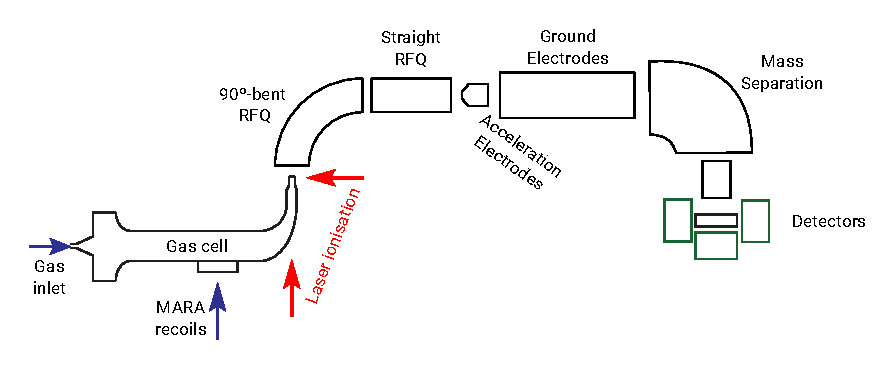
\includegraphics[scale=.8]{assets/LEB.pdf}}
    \end{textblock*}
    
     \begin{textblock*}{5cm}(1cm,5.5cm)
      \vspace{1em}
      \centering
      \textbf{Gas Cell}
      \flushleft
      \vspace{-0.6em}
      Recoils from MARA are stopped and neutralised in the gas cell using a buffer gas (He or Ar).
      
      They are evacuated using the gas flow and laser ionised inside the gas cell or in the gas jet.
    \end{textblock*}
        
    \begin{textblock*}{5cm}(7cm,5.5cm)
        \centering
        \vspace{1em}
        \textbf{Transport}
        \flushleft
        \vspace{-0.6em}
      Ions are transported to detector stations using ion optics.
      
      They are mass selected before the detector station via a dipole magnet.
    \end{textblock*}
\end{frame}

% \subsection{Vacuum Chambers}
\begin{frame}{VACUUM CHAMBERS}
    \begin{textblock*}{13cm}(0cm,1cm)
            \centering
            {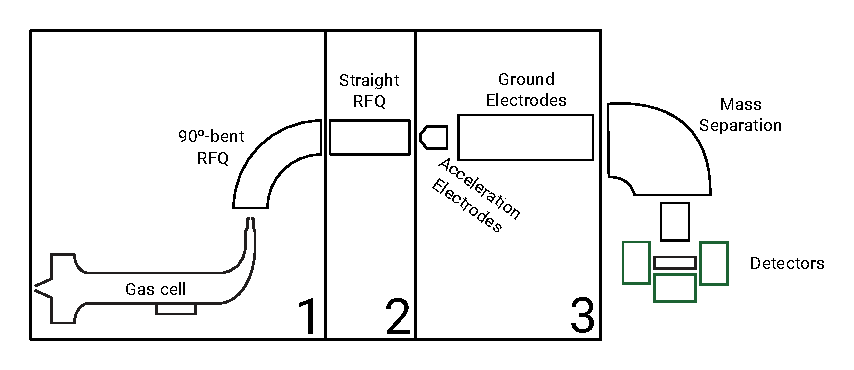
\includegraphics[scale=.8]{assets/LEBdiff.pdf}}
    \end{textblock*}
    
     \begin{textblock*}{5cm}(1.5cm,5.5cm)
      \vspace{2em}
      \onslide<1->{\textbf{Differential pumping section}}
        \begin{enumerate}
            \item<2-> Gas Cell Chamber
            \item<3-> Second Chamber
            \item<4-> Extraction Chamber
        \end{enumerate}
    \end{textblock*}
        
    \begin{textblock*}{5cm}(7cm,5.5cm)
        \vspace{2em}
        \centering
        \onslide<5->{\textbf{Other chambers are pumped regularly}}
    \end{textblock*}
\end{frame}

% \section{Vacuum System}
\subsection{The Facility}
\begin{frame}{VACUUM SYSTEM}
    \begin{textblock*}{13cm}(0cm,1cm)
            \centering
            {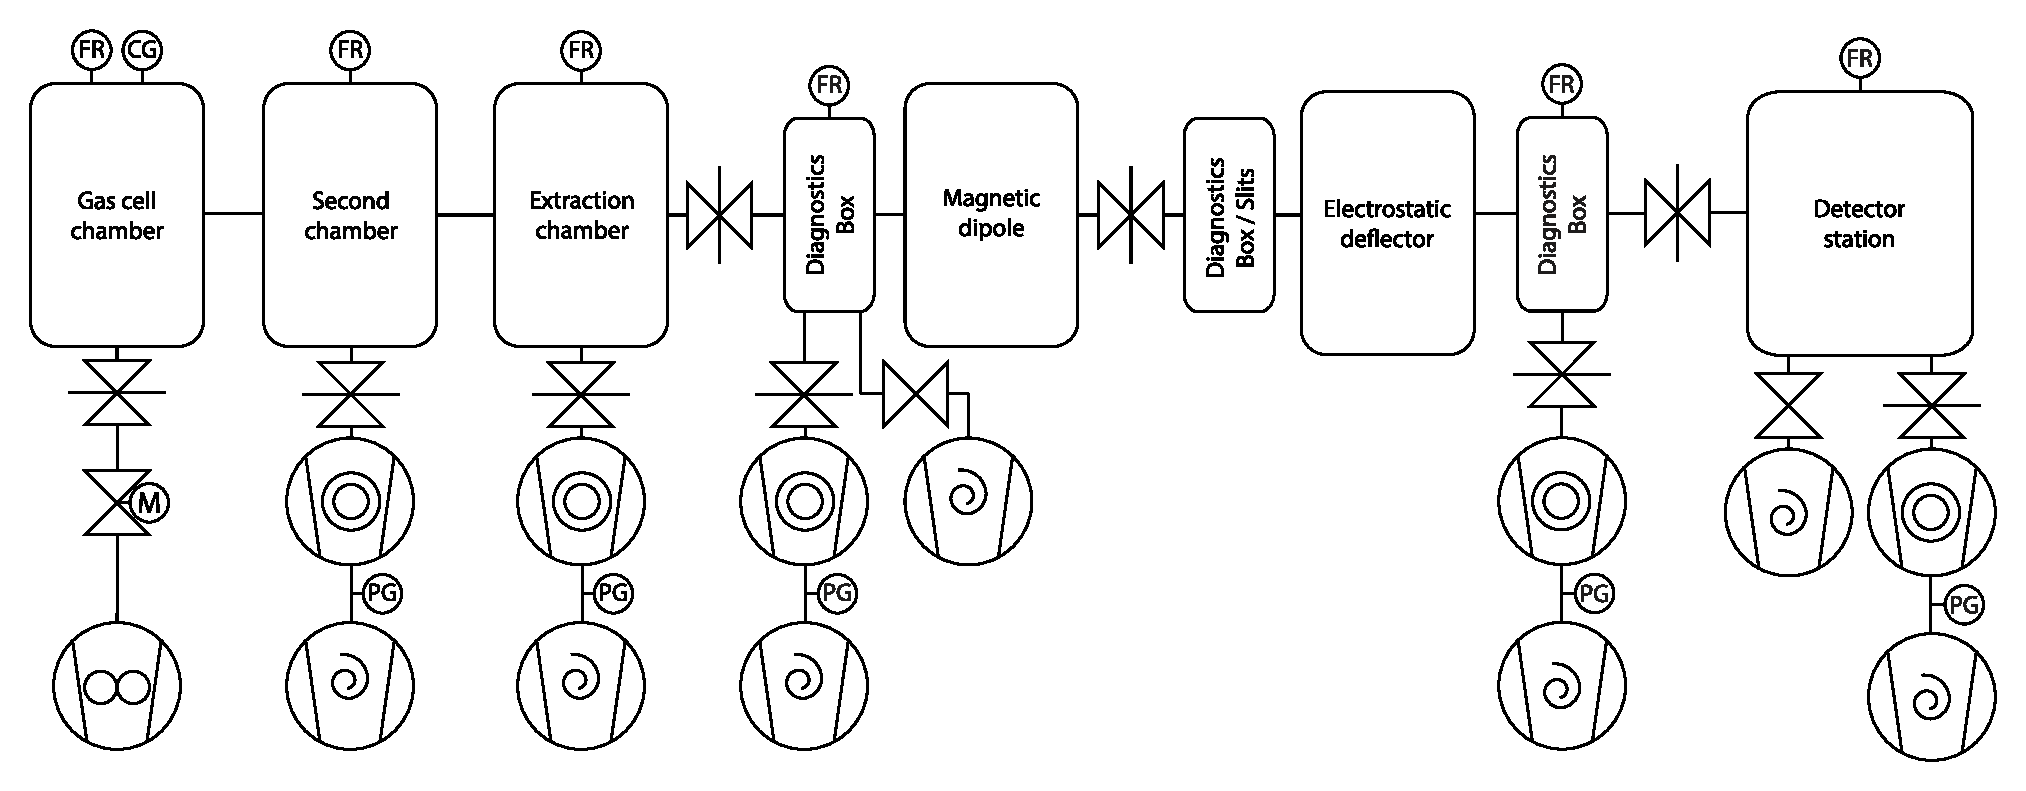
\includegraphics[scale=0.35]{assets/pumpdia.pdf}}
    \end{textblock*}
    
    \begin{textblock*}{5cm}(.5cm,6cm)
        \centering
        \textbf{Connection to MARA} 
      
      {MARA is kept at high vacuum, so the gas cell needs a thin window that can withstand pressure differences of up to $\sim$1E10\,mbar, but not stop recoils before entering the cell.}
    \end{textblock*}
    
    \begin{textblock*}{6.5cm}(6.5cm,5.5cm)
      \centering
            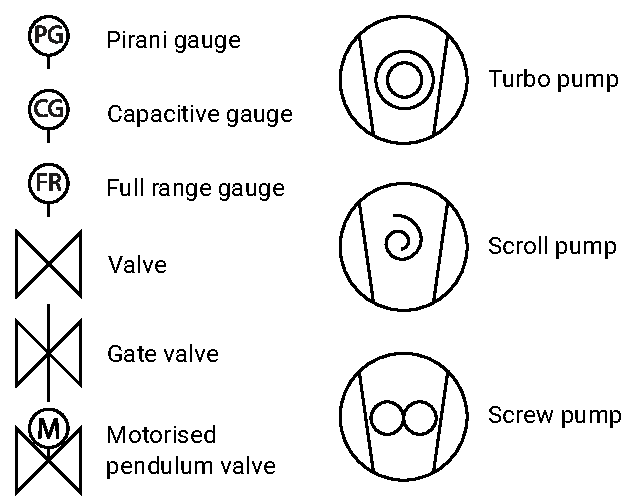
\includegraphics[scale=0.4]{assets/legend.pdf}
    \end{textblock*}
\end{frame}

% \subsection{Differential Pumping}
\begin{frame}{DIFFERENTIAL PUMPING}
    \begin{textblock*}{13cm}(0cm,1cm)
            \centering
            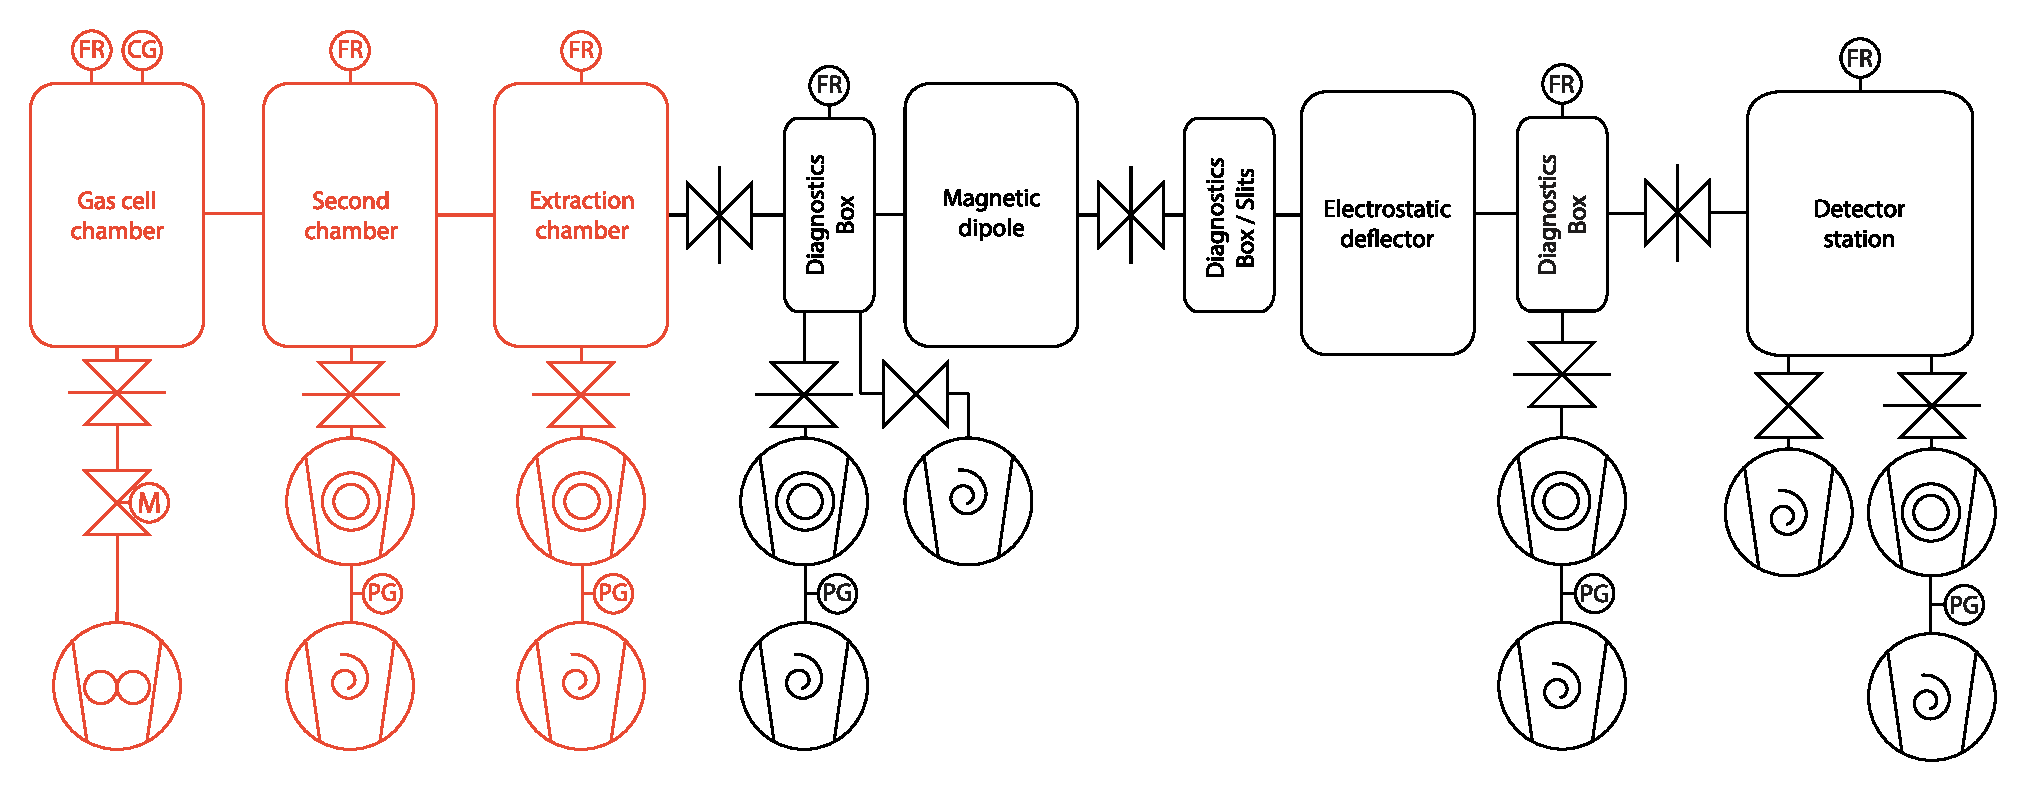
\includegraphics[scale=0.35]{assets/pumpdia2.pdf}
    \end{textblock*}
        
    \begin{textblock*}{5cm}(0.5cm,5.5cm)
      \centering
      \vspace{1em}
      \textbf{\color[RGB]{233,74,53} Differential pumping section} 
      
      {\color[RGB]{233,74,53} The gas cell chamber is going to have a constant inflow of gas, thus needing more powerful pump and valves that allow for the regulation of the gas flow into the screw pump.}
    \end{textblock*}
        
    \begin{textblock*}{5cm}(7.25cm,5.5cm)
        \centering
        \vspace{1em}
        \textbf{Normal pumping section} 
      
      {Thanks to the gate valves, entire sections of the beamline can be pumped separately and isolated to open other sections.}
    \end{textblock*}
\end{frame}


\begin{frame}{DIFFERENTIAL PUMPING}
    \begin{textblock*}{13cm}(0cm,1cm)
            \centering
            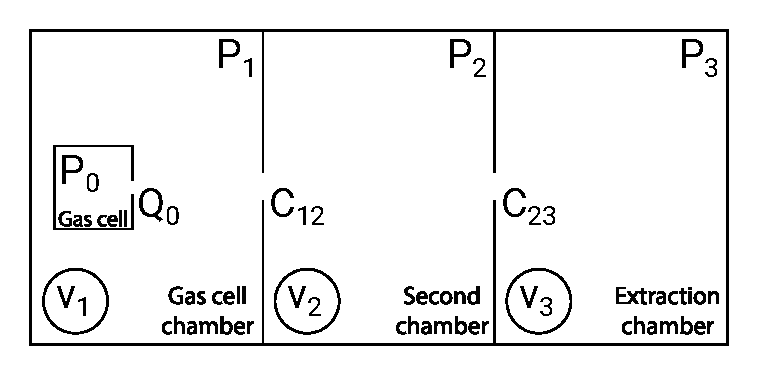
\includegraphics[scale=0.7]{assets/simpdiffsect.pdf}
    \end{textblock*}
    
    \begin{textblock*}{5cm}(1cm,5.5cm)
      \centering
      {\textbf{Apertures and Pipes}
      \begin{itemize}
          \item A$_0$: d = 0.5 - 1.2\,mm
          \item A$_{12}$: d = 5\,mm, $\ell$ = 10\,cm
          \item A$_{23}$: d = 5\,mm, $\ell$ = 10\,cm
      \end{itemize}}
    \end{textblock*}
    
    \begin{textblock*}{5cm}(7cm,5.5cm)
      \centering
      {\transparent{0.25}\textbf{Physical Properties}
        \begin{itemize}
          \item Volumes = 100\,L
          \item Surface area = 1.2\,m$^2$
          \item Outgassing = 1.8E-7\,mbar\,L/s/cm$^2$
        \end{itemize}}
    \end{textblock*}
    \end{frame}
    
\begin{frame}{DIFFERENTIAL PUMPING}
    \begin{textblock*}{13cm}(0cm,1cm)
            \centering
            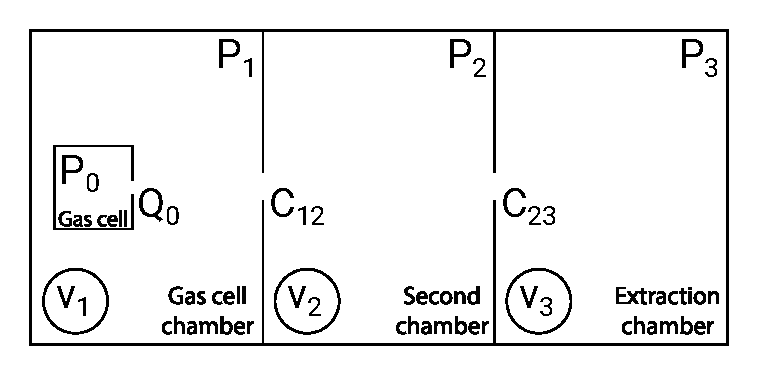
\includegraphics[scale=0.7]{assets/simpdiffsect.pdf}
    \end{textblock*}
    
    \begin{textblock*}{5cm}(1cm,5.5cm)
      \centering
      {\transparent{0.25} \textbf{Apertures and Pipes}
      \begin{itemize}
          \item A$_0$: d = 0.5 - 1.2\,mm
          \item A$_{12}$: d = 5\,mm, $\ell$ = 10\,cm
          \item A$_{23}$: d = 5\,mm, $\ell$ = 10\,cm
      \end{itemize}}
    \end{textblock*}
    
    \begin{textblock*}{5cm}(7cm,5.5cm)
      \centering
      {\transparent{1}\textbf{Physical Properties}
        \begin{itemize}
          \item Volumes = 100\,L
          \item Surface area = 1.2\,m$^2$
          \item Outgassing = 1.8E-7\,mbar\,L/s/cm$^2$
        \end{itemize}}
    \end{textblock*}
\end{frame}

\begin{frame}{DIFFERENTIAL PUMPING}
    \begin{textblock*}{13cm}(0cm,1cm)
            \centering
            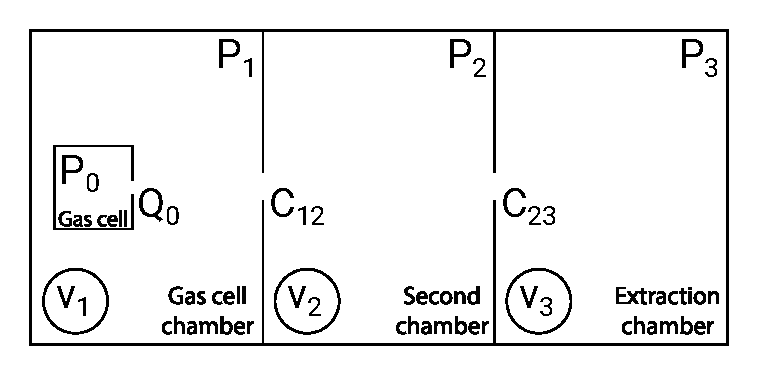
\includegraphics[scale=0.7]{assets/simpdiffsect.pdf}
    \end{textblock*}
    
    \begin{textblock*}{5cm}(1cm,5.5cm)
      \centering
      {\transparent{1} \textbf{Pumping Speeds}
      \begin{itemize}
          \item v$_1$ = 1056\,L/s (Screw)
          \item v$_2$ = 2000\,L/s (Turbo)
          \item v$_3$ = 1000\,L/s (Turbo)
      \end{itemize}}
    \end{textblock*}
    
    \begin{textblock*}{5cm}(7cm,5.5cm)
      \centering
      {\transparent{0.25} \textbf{Gas Cell Load}
        \begin{itemize}
          \item Q$_0$(He) = 55-650\,mbar\,L/s
          \item Q$_0$(Ar) = 20-200\,mbar\,L/s
        \end{itemize}\textbf{Leak Loads}
        \begin{itemize}
          \item Q$_{leak}$ = 1E-7 mbar\,L/s
        \end{itemize}}
    \end{textblock*}
\end{frame}

\begin{frame}{DIFFERENTIAL PUMPING}
    \begin{textblock*}{13cm}(0cm,1cm)
            \centering
            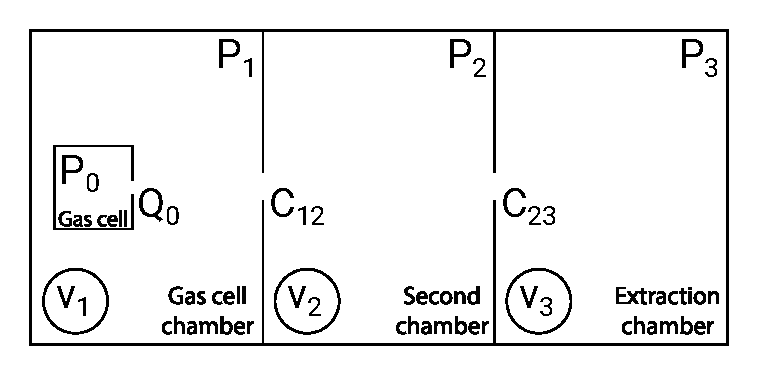
\includegraphics[scale=0.7]{assets/simpdiffsect.pdf}
    \end{textblock*}
    
    \begin{textblock*}{5cm}(1cm,5.5cm)
      \centering
      {\transparent{0.25} \textbf{Pumping Speeds}
      \begin{itemize}
          \item v$_1$ = 1056\,L/s (Screw)
          \item v$_2$ = 2000\,L/s (Turbo)
          \item v$_3$ = 1000\,L/s (Turbo)
      \end{itemize}}
    \end{textblock*}
    
    \begin{textblock*}{5cm}(7cm,5.5cm)
      \centering
      {\transparent{1} \textbf{Gas Cell Load}
        \begin{itemize}
          \item Q$_0$(He) = 55-650\,mbar\,L/s
          \item Q$_0$(Ar) = 20-200\,mbar\,L/s
        \end{itemize}\textbf{Leak Loads}
        \begin{itemize}
          \item Q$_{leak}$ = 1E-7 mbar\,L/s
        \end{itemize}}
    \end{textblock*}
\end{frame}

\begin{frame}{DIFFERENTIAL PUMPING}
    \begin{textblock*}{13cm}(0cm,1cm)
            \centering
            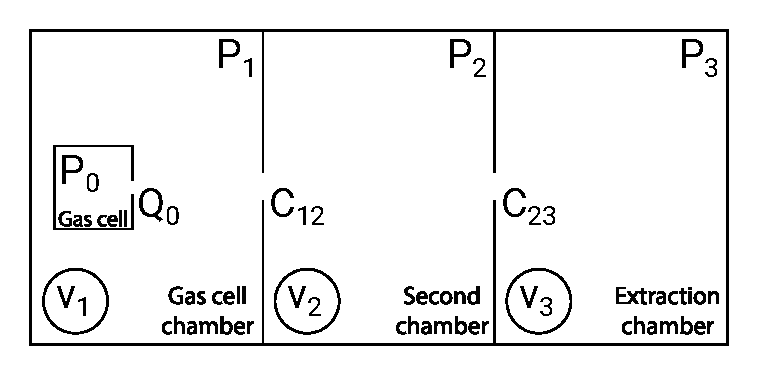
\includegraphics[scale=0.7]{assets/simpdiffsect.pdf}
    \end{textblock*}
    
    \begin{textblock*}{5cm}(1cm,5.5cm)
      \centering
      {\textbf{Target Pressures}
      \begin{itemize}
          \item P$_0$ = 500-1000\,mbar (He or Ar)
          \item P$_1$ $\simeq$ 0.01 - 0.1\,mbar
          \item P$_2$ $\simeq$ 10E-6 - 0.01\,mbar
          \item P$_3$ $\simeq$ 10E-6\,mbar
      \end{itemize}}
    \end{textblock*}
    
    \end{frame}

\begin{frame}{COMPARISON}
    \centering
    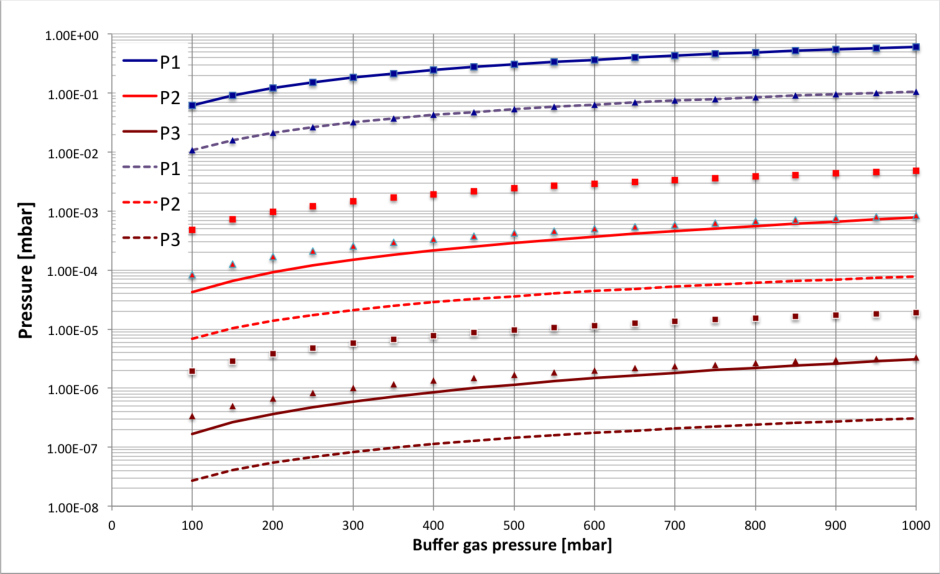
\includegraphics[scale=0.7]{assets/he_fin.pdf}
    \begin{textblock*}{11cm}(1.5cm,8.35cm)
    \begin{columns}
        \begin{column}{0.5\textwidth}
            \textbf{Square} = Aperture + d$_0$=1.2\,mm
            
            \textbf{Triangle} = Aperture + d$_0$=0.5\,mm
        \end{column}
        \begin{column}{0.5\textwidth}  %%<--- here
            \textbf{Solid Line} = Pipe + d$_0$=1.2\,mm
            
            \textbf{Dashed Lin}e = Pipe + d$_0$=0.5\,mm
        \end{column}
    \end{columns}
    \end{textblock*}
\end{frame}
\end{document}